\documentclass[12pt, a4paper]{article}

\usepackage[utf8]{inputenc}
\usepackage[spanish]{babel}
\usepackage{geometry}
\usepackage{titlesec}
\usepackage{enumitem}
\usepackage{xcolor}
\usepackage{listings}
\usepackage{mdframed}
\usepackage{hyperref}
\usepackage{tikz}
\usetikzlibrary{shapes.geometric, arrows.meta, positioning}

\geometry{margin=2.5cm}

% Colores
\definecolor{azulprincipal}{RGB}{30, 90, 160}
\definecolor{amarillopendiente}{RGB}{255, 200, 0}
\definecolor{grisclaro}{RGB}{245, 245, 245}
\definecolor{codigofondo}{RGB}{240, 244, 250}
\definecolor{codigoborde}{RGB}{30, 90, 160}

% Estilo de secciones
\titleformat{\section}{\large\bfseries\color{azulprincipal}}{}{0em}{}[\titlerule]
\titleformat{\subsection}{\normalsize\bfseries\color{azulprincipal}}{}{0em}{}

% Estilo de código inline
\lstset{
    basicstyle=\ttfamily\small,
    backgroundcolor=\color{codigofondo},
    frame=single,
    rulecolor=\color{codigoborde},
    breaklines=true,
    language=Java,
    keywordstyle=\color{azulprincipal}\bfseries,
    commentstyle=\color{gray},
    stringstyle=\color{teal},
}

% Caja de "pendiente"
\newmdenv[
    backgroundcolor=amarillopendiente!25,
    linecolor=amarillopendiente!80!black,
    leftmargin=0, rightmargin=0,
    innerleftmargin=8pt, innerrightmargin=8pt,
    innertopmargin=6pt, innerbottommargin=6pt,
    roundcorner=4pt
]{pendiente}

% --------------------------------------------------
\begin{document}

\begin{center}
    {\LARGE \textbf{Documentación: Patrón MVC + Observer}}\\[0.4em]
    {\large \textit{Space Invaders — Proyecto de Programación}}\\[0.3em]
    {\small Fecha: \today}
\end{center}

\vspace{0.5em}
\hrule
\vspace{1.5em}

% ==================================================
\tableofcontents
\newpage

% ==================================================
\section{Introducción al Patrón MVC + Observer}

El patrón \textbf{Modelo-Vista-Controlador (MVC)} es una arquitectura de diseño utilizada en programación orientada a objetos que permite organizar una aplicación separando sus componentes en tres partes principales: \textit{Modelo}, \textit{Vista} y \textit{Controlador}. Esta separación facilita el mantenimiento del código, mejora su organización y permite que cada componente tenga una responsabilidad clara dentro del sistema.

\begin{description}[leftmargin=2em, style=nextline]
    \item[\textbf{Modelo}]
        Se encarga de gestionar los datos y la lógica del programa. Contiene toda la lógica de negocio, del juego en este caso, y las operaciones necesarias para modificarla o consultarla. El modelo no depende de la interfaz gráfica ni de cómo se muestran los datos al usuario.

    \item[\textbf{Vista}]
        Es la parte encargada de presentar la información al usuario. Su función principal es mostrar los datos que proporciona el modelo y actualizarse cuando estos cambian. La vista no contiene la lógica principal del programa, sino únicamente la representación visual de la información.

    \item[\textbf{Controlador}]
        Actúa como intermediario entre el usuario y el sistema. Recibe las acciones del usuario (por ejemplo, clics, entradas de teclado, etc.), interpreta estas acciones y solicita al modelo que realice las operaciones correspondientes.
\end{description}

A este modelo de arquitectura se le añade el patrón \textbf{Observer (Observador)} para que la vista se mantenga actualizada cuando cambian los datos del modelo. Este \textbf{patrón de diseño} establece una relación entre un objeto denominado \textit{observable} (el modelo) y uno o varios \textit{observadores} (las vistas). Cuando el estado del observable cambia, todos los observadores registrados son notificados automáticamente y pueden actualizar su información.


La combinación de MVC y Observer permite desarrollar aplicaciones más modulares, donde la lógica del programa, la presentación de los datos y la interacción con el usuario están claramente separadas. Esto facilita la reutilización del código, la ampliación del sistema y el mantenimiento a largo plazo de la aplicación.

% ==================================================
\section{Implementación en Space Invaders}

% --------------------------------------------------
\subsection{Arquitectura MVC del proyecto}

En el proyecto Space Invaders, las tres capas del patrón MVC se distribuyen de la siguiente manera:

\begin{description}[leftmargin=2em, style=nextline]
    \item[\textbf{Modelo}]
        La clase central del modelo es \texttt{Espacio}, que está implementado como \textbf{Singleton} y extiende de la clase \texttt{Observable}. Contiene toda la lógica del juego: la instancia del \texttt{Jugador}, la lista de \texttt{Enemigo}s y el objeto \texttt{Disparo} asociado al jugador. Además, \texttt{Espacio} alberga el bucle principal del juego (\textit{game loop} con un \texttt{Timer} de 50 ms), la detección de colisiones entre el disparo y los enemigos, y las condiciones de fin de partida (\textit{game over} y victoria).

        Las clases auxiliares del modelo definen la estructura de las naves y los disparos del juego:
        \begin{itemize}[leftmargin=2em]
            \item \texttt{Naves} — clase abstracta que encapsula el comportamiento común de todas las naves. Define atributos: \texttt{x} (posición horizontal), \texttt{y} (posición vertical), \texttt{velocidad} (píxeles por actualización, por defecto 1) y \texttt{vivo} (estado actual). Incluye el método abstracto \texttt{mover()}, que cada subclase implementa según su lógica de movimiento. \textbf{Nota:} El atributo \texttt{velocidad} solo lo utiliza la clase \texttt{Jugador}; la clase \texttt{Enemigo} no lo usa.
            \item \texttt{Jugador} — extiende \texttt{Naves} y representa la nave controlable. Implementa \texttt{mover()} multiplicando los desplazamientos por \texttt{velocidad}, permitiendo movimiento dentro de los límites del tablero visible (0-99 en x, 0-59 en y). Posee un objeto \texttt{Disparo} que se dispara cuando el usuario presiona espacio. Solo hay una instancia del jugador simultáneamente y solo un disparo activo por jugador.
            \item \texttt{Enemigo} — extiende \texttt{Naves} y representa un enemigo del juego. Implementa \texttt{mover()} sumando directamente los desplazamientos sin usar \texttt{velocidad}. Se crean inicialmente en una posición aleatoria en la fila superior (y entre 0-4) y descienden verticalmente. Se eliminan al salir del tablero o ser impactados por un disparo. El juego comienza con un único enemigo.
            \item \texttt{Disparo} — representa el proyectil disparado por el jugador. Almacena su posición actual (\texttt{x}, \texttt{y}) y un booleano (\texttt{activo}) para saber si está en vuelo. Se crea un nuevo \texttt{Disparo} cada vez que el jugador presiona espacio, con posición inicial \texttt{(x\_jugador, y\_jugador - 1)}, reemplazando el anterior. Asciende un píxel por tick (cada 50ms) mediante el método \texttt{subir()}. Se desactiva automáticamente cuando alcanza y<0 (sale del tablero).
        \end{itemize}

        Ninguna de estas clases conoce la interfaz gráfica ni sabe cómo se dibuja el juego; solo gestionan datos y reglas de juego.

    \item[\textbf{Vista}]
        Las vistas son \texttt{StartFrame} y \texttt{MainFrame}, ambas subclases de \texttt{JFrame} e implementan la interfaz \texttt{Observer}. Su función es capturar el estado del modelo y representarlo visualmente sin contener lógica de negocio:
        \begin{itemize}[leftmargin=2em]
            \item \texttt{StartFrame} es la pantalla inicial del juego. Se encarga de mostrar el título ("SPACE INVADERS"), el subtítulo ("Sprint 1"), las instrucciones básicas de control, y el mensaje «Pulsa SPACE para jugar». No dibuja ningún elemento del juego ni gestiona la lógica de juego. Su responsabilidad es permitir que el usuario active el inicio de la partida.
            \item \texttt{MainFrame} es la pantalla de juego principal y gestiona toda la representación gráfica. Usa una matriz de \texttt{JLabel}s para representar el tablero como cuadrícula negra de $100 \times 60$ celdas (cada celda de $10 \times 10$ píxeles). Los elementos se representan con colores: el jugador como celdas magenta, los enemigos como celdas rojas, y el disparo como celda amarilla. También muestra un mensaje de victoria o derrota cuando la partida termina.
        \end{itemize}

        El mecanismo clave es que ambas vistas se registran automáticamente como observadoras de \texttt{Espacio} al construirse, mediante la llamada \lstinline|Espacio.getEspacio().addObserver(this)| en sus constructores. Esto garantiza que recibirán notificaciones automáticas de cualquier cambio en el estado del juego.

    \item[\textbf{Controlador}]
        Los controladores son clases internas privadas llamadas \texttt{Controller} definidas dentro de \texttt{StartFrame} y \texttt{MainFrame}. Ambas implementan \texttt{KeyListener}, lo que requiere implementar obligatoriamente los tres métodos de la interfaz: \texttt{keyPressed}, \texttt{keyReleased} y \texttt{keyTyped}. En la práctica, solo \texttt{keyPressed} contiene lógica (los otros dos están vacíos). Esto permite que el controlador reciba los eventos del teclado, interprete las teclas pulsadas y traduzca en llamadas concretas al modelo:
        \begin{itemize}[leftmargin=2em]
            \item El \texttt{Controller} de \texttt{StartFrame} escucha la pulsación de \texttt{SPACE} para llamar a \lstinline|Espacio.getEspacio().cambiarAMain()|, indicando al modelo que inicie la partida.
            \item El \texttt{Controller} de \texttt{MainFrame} atiende las cuatro flechas direccionales (llamando a \lstinline|espacio.moverJugador(dx, dy)| con los desplazamientos) y la barra espaciadora (llamando a \lstinline|espacio.disparar()|). La verificación de si la partida ha terminado \textbf{no está en el Controller}, sino en el \textbf{modelo} (en los métodos \texttt{moverJugador()} y \texttt{disparar()}).
        \end{itemize}
\end{description}

La relación entre las tres capas queda así: el usuario interactúa con la \textbf{Vista} (ventana con foco de teclado), el \textbf{Controlador} captura esa interacción y llama al \textbf{Modelo}, y el Modelo notifica a la Vista para que se hagan los cambios necesarios. En ningún momento la vista accede directamente a la lógica del juego, ni el modelo sabe cómo se representa gráficamente.

Más adelante se verá como se implementa esta relación entre las tres capas en el proyecto Space Invaders.

% --------------------------------------------------
\subsection{Diagramas UML}

\begin{figure}[h]
    \centering
    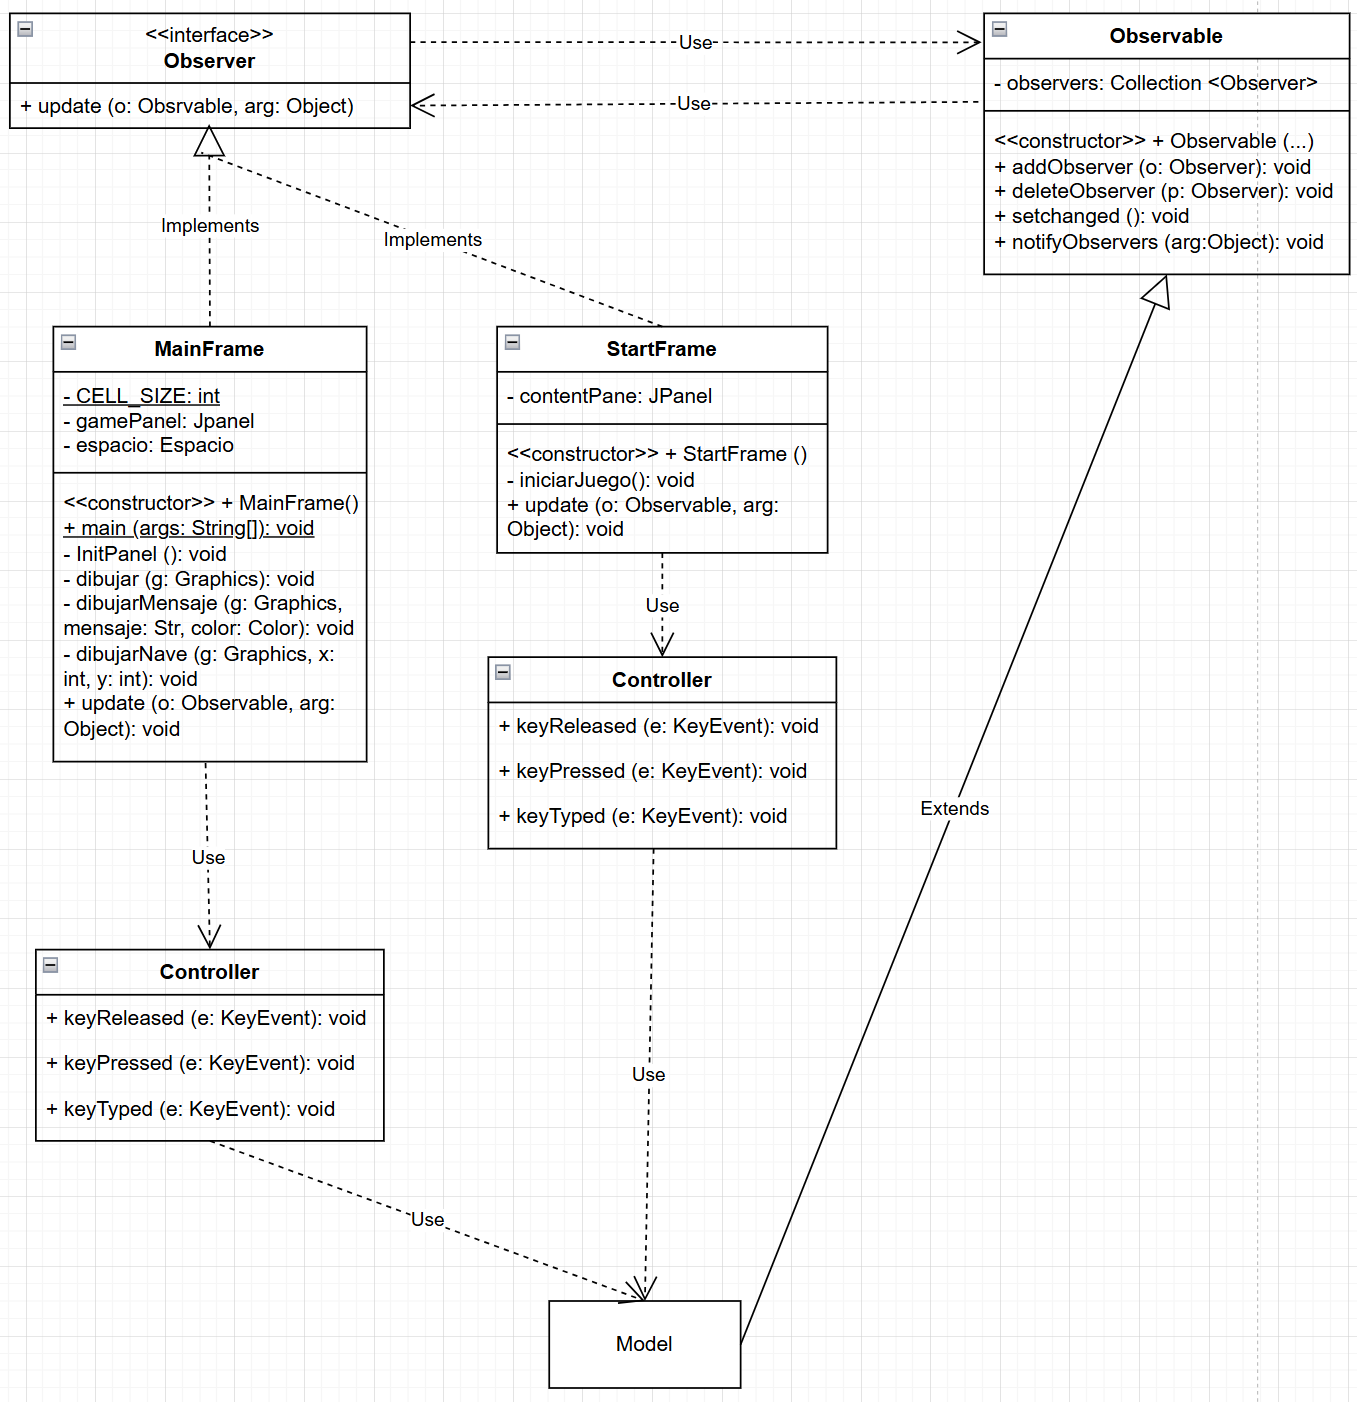
\includegraphics[width=1.0\textwidth]{VistaController.png}
    \caption{Diagrama UML de la arquitectura MVC y relación Observer entre las clases del proyecto Space Invaders.}
    \label{fig:mvc_observer}
\end{figure}

% ==================================================
\section{El Controlador en Detalle}

El controlador es el intermediario entre el usuario y el sistema. Recibe las acciones del usuario (eventos de teclado), las interpreta según la lógica de control definida, y solicita al modelo que execute las operaciones correspondientes. No contiene datos del juego ni se encarga de mostrarlos; simplemente traduce entrada en acciones del modelo.

% --------------------------------------------------
\subsection{Método \texttt{notificarInicializacion}}

Este método es crucial para inicializar la pantalla de juego correctamente. Se llama desde el constructor de \texttt{MainFrame} después de que toda la interfaz gráfica está lista.

\begin{lstlisting}
public void notificarInicializacion() {
    setChanged();
    notifyObservers(new int[] {6, jugador.getX(), jugador.getY(), 
                               enemigos.get(0).getX(), enemigos.get(0).getY()});
}
\end{lstlisting}

Envía una notificación de tipo 6 con las posiciones iniciales del jugador y el primer enemigo. Esto permite que \texttt{MainFrame} pinte estos elementos en el tablero sin necesidad de que ocurra movimiento alguno.

% --------------------------------------------------
\subsection{Método \texttt{cambiarAMain}}

Este método realiza tres tareas críticas:

\begin{lstlisting}
public void cambiarAMain() {
    inicializar();           // Crear jugador y primer enemigo
    iniciarJuegoLoop();      // Iniciar el timer de 50ms
    setChanged();
    notifyObservers(new int[] {9}); // Notificación para cambiar de pantalla
}
\end{lstlisting}

\begin{enumerate}[leftmargin=2em]
    \item \textbf{Inicializar}: Crea la instancia del \texttt{Jugador} en posición (50, 55) y añade el primer \texttt{Enemigo} en una posición aleatoria en la fila superior (y entre 0-4).
    \item \textbf{Iniciar game loop}: Arranca el \texttt{Timer} de 50 ms que ejecutará el bucle principal del juego.
    \item \textbf{Notificar}: Envía notificación tipo 9 para que \texttt{StartFrame} cierre y \texttt{MainFrame} se abra.
\end{enumerate}

\subsubsection*{Clase \texttt{MainFrame}}

El \texttt{Controller} de esta clase es la parte que traduce las teclas del usuario en acciones del juego. Está definido como una clase interna en \texttt{MainFrame} e implementa \texttt{KeyListener}, por lo que escucha eventos del teclado.

Su flujo es el siguiente:

\begin{enumerate}[leftmargin=2em]
    \item Se crea en \texttt{MainFrame} con \lstinline|Controller controller = new Controller()|.
    \item Se registra en la ventana con \lstinline|addKeyListener(...)| en \texttt{MainFrame}.
    \item Para que realmente reciba teclas, el frame solicita el foco en \texttt{MainFrame}.
\end{enumerate}

Lo importante ocurre en \texttt{keyPressed} en \texttt{MainFrame}:

\begin{itemize}[leftmargin=2em]
    \item Lee qué tecla se pulsó con \lstinline|e.getKeyCode()|.
    \item Según la tecla, llama al modelo \texttt{Espacio}:
    \begin{itemize}[leftmargin=2em]
        \item \textbf{Flecha izquierda:} ejecuta \lstinline|espacio.moverJugador(-1, 0)|.
        \item \textbf{Flecha derecha:} ejecuta \lstinline|espacio.moverJugador(1, 0)|.
        \item \textbf{Flecha arriba:} ejecuta \lstinline|espacio.moverJugador(0, -1)|.
        \item \textbf{Flecha abajo:} ejecuta \lstinline|espacio.moverJugador(0, 1)|.
        \item \textbf{Espacio:} ejecuta \lstinline|espacio.disparar()|.
    \end{itemize}
\end{itemize}

Importante: El \texttt{Controller} \textbf{no verifica} si la partida ha terminado. Esa validación ocurre dentro del modelo en los métodos \texttt{moverJugador()} y \texttt{disparar()}, que comprueban internamente con \lstinline|isGameOver()| y \lstinline|isGameWon()| antes de ejecutar.

En resumen: el \texttt{Controller} no contiene lógica de juego ni dibuja nada; solo captura la entrada del teclado y translada a llamadas de modelo. El modelo valida y ejecuta. Después, cuando el modelo notifica a la vista, el método \texttt{update} actualiza el panel gráfico.

\subsubsection*{Clase \texttt{StartFrame}}

En esta clase, el \texttt{Controller} sirve para controlar la pantalla de inicio usando el teclado. Está definido al final de \texttt{StartFrame} como una clase interna que implementa \texttt{KeyListener}.

Su función es muy simple: escuchar si el usuario pulsa la barra espaciadora.

El flujo es el siguiente:

\begin{enumerate}[leftmargin=2em]
    \item En el constructor de \texttt{StartFrame} se crea el controller e inmediatamente se registra con \lstinline|addKeyListener(controller)|.
    \item La ventana pide el foco con \lstinline|requestFocusInWindow()|, por lo que puede recibir eventos del teclado.
    \item Cuando el usuario pulsa una tecla, se ejecuta \texttt{keyPressed} en el \texttt{Controller}.
\end{enumerate}

Dentro de \texttt{keyPressed}, el controller hace una sola comprobación:

\begin{itemize}[leftmargin=2em]
    \item Si la tecla pulsada es \texttt{VK\_SPACE}, llama a \lstinline|iniciarJuego()| que a su vez llama a \lstinline|Espacio.getEspacio().cambiarAMain()|.
\end{itemize}

Ese método \texttt{cambiarAMain()} en \texttt{Espacio} dispara todo el proceso de transición en cascada: inicializa el juego, arranca el timer, y notifica a los observers. Como \texttt{StartFrame} es una de los observadores, su método \texttt{update} recibe la notificación de tipo 9 y cierra la ventana de inicio.

% ==================================================
\section{Patrón Observer: Notificación y Actualización}

Dentro del patrón Observer, los métodos \texttt{notify} y \texttt{update} permiten que los objetos que observan a otro objeto puedan mantenerse informados cuando su estado cambia.

% --------------------------------------------------
\subsection{Método \texttt{notify}}

El método \texttt{notify} pertenece al objeto \textbf{observable}, que es el objeto que contiene los datos o el estado que puede cambiar. En muchas aplicaciones que siguen la arquitectura MVC, el observable suele ser el modelo, ya que es el componente que gestiona la información y la lógica del sistema.

La función del método \texttt{notify} es avisar a todos los observadores registrados de que el estado del observable ha cambiado. Para ello, el observable mantiene normalmente una lista o colección de observadores que se han registrado previamente para recibir notificaciones.

Cuando ocurre un cambio relevante en el estado del observable (por ejemplo, una modificación de datos), el método \texttt{notify} recorre esta lista de observadores y llama al método \texttt{update} de cada uno de ellos. De esta manera, todos los observadores reciben la notificación del cambio y pueden reaccionar en consecuencia.

Una característica importante del método \texttt{notify} es que el observable \textbf{no necesita conocer los detalles internos de los observadores}. Simplemente se encarga de avisarlos de que ha ocurrido un cambio. Esto permite mantener un bajo acoplamiento entre las clases, lo que facilita la reutilización del código y el mantenimiento del sistema.

% --------------------------------------------------
\subsection{Método \texttt{update}}

El método \texttt{update} pertenece a los \textbf{observadores}. Cada observador debe implementar este método para definir cómo reaccionará cuando el observable le notifique un cambio.

Cuando el observable ejecuta el método \texttt{notify}, este llama al método \texttt{update} de cada observador registrado. En ese momento, el observador recibe la notificación y puede realizar las acciones necesarias para actualizar su estado.

En muchos casos, el método \texttt{update} se utiliza para que el observador consulte el nuevo estado del observable y adapte su comportamiento o su representación visual. Por ejemplo, si el observable es el modelo de una aplicación y el observador es una vista, el método \texttt{update} se encargará de actualizar la información que se muestra al usuario para reflejar los cambios recientes.

Cada observador puede implementar su propio comportamiento en el método \texttt{update}, lo que permite que diferentes componentes reaccionen de distintas formas ante el mismo cambio en el observable.

% --------------------------------------------------
\subsection{Funcionamiento conjunto de \texttt{notify} y \texttt{update}}

El funcionamiento coordinado de estos dos métodos permite mantener sincronizados los distintos componentes de un sistema que utiliza el patrón Observer. El proceso general es el siguiente:

\begin{enumerate}[leftmargin=2em]
    \item Se produce un cambio en el estado del objeto observable.
    \item El observable detecta ese cambio y ejecuta el método \texttt{notify}.
    \item El método \texttt{notify} recorre la lista de observadores registrados.
    \item Para cada observador, se llama a su método \texttt{update}.
    \item Cada observador recibe la notificación y actualiza su estado o su información según corresponda.
\end{enumerate}

Gracias a este mecanismo, los cambios en el sistema se propagan automáticamente a los objetos que dependen de ellos, sin necesidad de que exista una dependencia directa entre todas las clases.

% --------------------------------------------------
\subsection{Aplicación al proyecto Space Invaders}

\subsubsection{Quién notifica y cuándo}

En el proyecto, el observable es \texttt{Espacio}. Las notificaciones a los observadores se realizan directamente con la secuencia:

\begin{lstlisting}
setChanged();
notifyObservers(new int[] {tipo, datos...});
\end{lstlisting}

La llamada a \lstinline|setChanged()| es obligatoria antes de \lstinline|notifyObservers()|: sin ella, la clase \texttt{Observable} no propagar\u00eda nada. \texttt{notifyObservers()} recorre internamente la lista de observers registrados y llama al \texttt{update} de cada uno, pasando un array de enteros con información espec\u00edfica sobre el cambio.

Las notificaciones se invocan desde varios puntos del modelo, cada vez que el estado del juego cambia y la pantalla debe reflejarlo. Los tipos de notificación (primer elemento del array) son:

\begin{itemize}[leftmargin=2em]
    \item \textbf{Tipo 0: Movimiento del jugador} — dentro de \texttt{moverJugador()}, tras actualizar la posición. Array: \lstinline|{0, oldX, oldY, newX, newY}|
    \item \textbf{Tipo 1: Nuevo disparo} — dentro de \texttt{disparar()}, tras crear un nuevo \texttt{Disparo}. Array: \lstinline|{1, newX, newY}|
    \item \textbf{Tipo 2: Movimiento del disparo} — dentro de \texttt{actualizarDisparo()}, en cada tick del \textit{game loop} (cada 50 ms) mientras el proyectil está activo. Array: \lstinline|{2, oldX, oldY, newX, newY}|
    \item \textbf{Tipo 3: Disparo sale del tablero} — dentro de \texttt{actualizarDisparo()}, cuando el disparo alcanza y=0. Array: \lstinline|{3, oldX, oldY}|
    \item \textbf{Tipo 4: Movimiento de enemigo} — dentro de \texttt{actualizarEnemigos()}, cada 200 ms (cada 4 ticks de 50ms), tras desplazar un enemigo. Array: \lstinline|{4, oldX, oldY, newX, newY}|
    \item \textbf{Tipo 5: Colisión disparo-enemigo} — dentro de \texttt{comprobarColisiones()}, cuando el disparo alcanza a un enemigo. Array: \lstinline|{5, disparoX, disparoY, enemigoX, enemigoY}|
    \item \textbf{Tipo 6: Inicialización del juego} — dentro de \texttt{notificarInicializacion()}, al abrir \texttt{MainFrame}. Pinta el jugador y el \textbf{primer} enemigo del array. Array: \lstinline|{6, jugadorX, jugadorY, enemigoX, enemigoY}|
    \item \textbf{Tipo 7: Game Over} — dentro de \texttt{actualizarEnemigos()}, cuando se detecta que un enemigo ha llegado a la fila del jugador. Array: \lstinline|{7}|
    \item \textbf{Tipo 8: Victoria} — dentro de \texttt{comprobarColisiones()}, cuando se elimina el último enemigo vivo. Array: \lstinline|{8}|
    \item \textbf{Tipo 9: Cambio a MainFrame} — dentro de \texttt{cambiarAMain()}, para señalar que \texttt{StartFrame} debe ceder control a \texttt{MainFrame}. \textbf{Solo es procesado por StartFrame}, no por MainFrame. Array: \lstinline|{9}|
\end{itemize}

\subsubsection{Estructura de datos en las notificaciones}

Cada notificación es un array de enteros que comienza con un identificador de tipo (0-9) seguido de parámetros específicos:

\begin{description}[leftmargin=2em, style=nextline]
    \item[\textbf{Primer elemento (índice 0)}]
        Siempre es el tipo de notificación (0-9). Define qué acción ocurrió en el modelo.

    \item[\textbf{Elementos posteriores}]
        Dependen del tipo. Pueden ser coordenadas (x, y), posiciones anteriores y nuevas, o una combinación de ambas. La longitud del array varía según el tipo:
        \begin{itemize}[leftmargin=2em]
            \item Tipos 0, 2, 4: 5 elementos (tipo + 4 coordenadas: oldX, oldY, newX, newY)
            \item Tipos 1, 3: 3 elementos (tipo + 2 coordenadas: X, Y)
            \item Tipo 5: 5 elementos (tipo + posición disparo + posición enemigo)
            \item Tipo 6: 5 elementos (tipo + posición jugador + posición primer enemigo)
            \item Tipos 7, 8, 9: 1 elemento (solo el tipo)
        \end{itemize}
\end{description}

\textbf{Ejemplo práctico:} Cuando el jugador se mueve de (50, 55) a (51, 55) presionando flecha derecha, el modelo ejecuta:

\begin{lstlisting}
int oldX = 50, oldY = 55;  // Posición anterior
jugador.mover(1, 0);       // dx=1, dy=0 (flecha derecha)
int newX = jugador.getX(); // Ahora 51
int newY = jugador.getY(); // Sigue siendo 55
setChanged();
notifyObservers(new int[] {0, 50, 55, 51, 55});
\end{lstlisting}

Esta notificación se envía a ambos frames (\texttt{MainFrame} y \texttt{StartFrame}), pero solo \texttt{MainFrame} la procesa porque está en el juego principal.

\subsubsection{Cómo responde \texttt{MainFrame} en su \texttt{update}}

\texttt{MainFrame} implementa \texttt{Observer} y se registra en \texttt{Espacio} al construirse. Su método \texttt{update} procesa las notificaciones específicas:

\begin{lstlisting}
@Override
public void update(Observable o, Object arg) {
    if (o instanceof Espacio) {
        int[] datos = (int[]) arg;
        procesarNotificacion(datos);
    }
}
\end{lstlisting}

El método \texttt{procesarNotificacion} es un switch que analiza el primer elemento del array (el tipo de evento, del 0 al 8) y actualiza selectivamente las celdas en la matriz \texttt{celdas[x][y]} según el caso:

\begin{itemize}[leftmargin=2em]
    \item Borra posiciones anteriores estableciendo el color de fondo a negro.
    \item Pinta nuevas posiciones con el color correspondiente: magenta para el jugador, rojo para enemigos, amarillo para el disparo.
    \item Para tipos 7 y 8, muestra un mensaje de fin de partida ("GAME OVER" en rojo o "HAS GANADO!" en verde).
    \item \textbf{Nota:} El switch solo procesa tipos 0-8. Las notificaciones de tipo 9 no son procesadas aquí; solo \texttt{StartFrame} las maneja.
\end{itemize}

\textbf{Ejemplo de procesamiento en MainFrame:}

Cuando llega la notificación tipo 0 (movimiento del jugador) con array \lstinline|{0, 50, 55, 51, 55}|:

\begin{lstlisting}
// Dentro del switch de procesarNotificacion():
case 0: // jugador se mueve - [tipo, oldX, oldY, newX, newY]
    celdas[datos[1]][datos[2]].setBackground(COLOR_FONDO);      // datos[1]=50, datos[2]=55
    celdas[datos[3]][datos[4]].setBackground(COLOR_JUGADOR);    // datos[3]=51, datos[4]=55
    break;
\end{lstlisting}

Esto:
\begin{enumerate}[leftmargin=2em]
    \item Lee la celda en la posición anterior (50, 55).
    \item La pinta de color negro (fondo), borrando visualmente el jugador de ahí.
    \item Lee la celda en la nueva posición (51, 55).
    \item La pinta de color magenta, mostrando el jugador en su nueva ubicación.
\end{enumerate}

El resultado visual es instantáneo: el jugador desaparece de (50, 55) y reaparece en (51, 55).

Esta aproximación de actualización selectiva de celdas es más eficiente que repintar todo el tablero en cada cambio y permite actualizaciones visuales precisas.

Adicionalmente, en el constructor de \texttt{MainFrame} se llama a \lstinline|espacio.notificarInicializacion()| para que el modelo envíe una notificación tipo 6 con las posiciones iniciales del jugador y primer enemigo.

\subsubsection{Cómo responde \texttt{StartFrame} en su \texttt{update}}

\texttt{StartFrame} también implementa \texttt{Observer} y se registra en \texttt{Espacio} al construirse. Su método \texttt{update} tiene un comportamiento distinto: no dibuja nada, sino que gestiona la transición entre pantallas. \textbf{Es el único que procesa notificaciones de tipo 9}, que es la señal para cambiar a \texttt{MainFrame}:

\begin{lstlisting}
@Override
public void update(Observable o, Object arg) {
    int[] datos = (int[]) arg;
    int tipo = datos[0];
    if (o instanceof Espacio) {
        if (tipo == 9) {       // Solo reacciona a tipo 9
            Espacio.getEspacio().deleteObserver(this);
            this.setVisible(false);
            new MainFrame();
        }
        // Tipos 0-8 se ignoran completamente en StartFrame
    }
}
\end{lstlisting}

Cuando \texttt{Espacio} notifica con tipo 9 (lo que ocurre al llamar a \texttt{cambiarAMain()} desde el controlador de \texttt{StartFrame}), este \texttt{update}:
\begin{enumerate}[leftmargin=2em]
    \item Extrae el array de datos: \lstinline|int[] datos = (int[]) arg|
    \item Lee el tipo en \lstinline|datos[0]|, que es 9
    \item Verifica: ¿es este el evento que me interesa? (Solo tipo 9)
    \item Si es tipo 9, ejecuta el flujo de transición:
    \begin{enumerate}[leftmargin=2em]
        \item Se desregistra como observer con \lstinline|deleteObserver(this)|, para no recibir más notificaciones futuras del juego.
        \item Oculta la ventana de inicio con \lstinline|setVisible(false)|.
        \item Crea un nuevo \texttt{MainFrame}, que al construirse se registra automáticamente como observer de \texttt{Espacio} y abre la pantalla de juego.
    \end{enumerate}
\end{enumerate}

\textbf{Diferencia crítica entre frames:}

\begin{itemize}[leftmargin=2em]
    \item \texttt{MainFrame}: Recibe \textbf{todos} los tipos (0-8) y procesa cada uno en el switch. Ignora los tipos 9.
    \item \texttt{StartFrame}: Recibe \textbf{todos} los tipos, pero solo procesa tipo 9. Ignora todos los demás.
\end{itemize}

Este diseño es eficiente porque cada frame solo reacciona a lo que le es relevante, incluso aunque ambos sean observadores del mismo observable. No hay desperdicio de recursos procesando eventos que no interesan.

Además, un único evento de notificación tipo 9 actúa como señal de arranque coordinada: hace desaparecer la pantalla de inicio y aparece la pantalla de juego, sin que ninguna de las dos clases necesite conocerse directamente entre sí.

% ==================================================
\section{Conclusiones}

La implementación del patrón MVC junto con Observer en el proyecto Space Invaders demuestra las ventajas de una arquitectura bien estructurada:

\begin{itemize}[leftmargin=2em]
    \item \textbf{Separación clara de responsabilidades}: El modelo (\texttt{Espacio}) gestiona exclusivamente la lógica del juego, las vistas (\texttt{StartFrame}, \texttt{MainFrame}) se encargan únicamente de la presentación, y los controladores traducen la interacción del usuario en acciones del modelo.
    
    \item \textbf{Bajo acoplamiento}: Las clases no dependen directamente unas de otras. El modelo no conoce las vistas, y las vistas no contienen lógica de negocio.
    
    \item \textbf{Sincronización automática}: El patrón Observer garantiza que cualquier cambio en el modelo se refleje inmediatamente en todas las vistas registradas, sin necesidad de llamadas explícitas.
    
    \item \textbf{Facilidad de mantenimiento}: Los cambios en la lógica del juego solo afectan al modelo, los cambios en la interfaz solo afectan a las vistas, y las modificaciones en los controles solo afectan a los controladores.
    
    \item \textbf{Extensibilidad}: Es fácil añadir nuevas vistas (por ejemplo, una pantalla de puntuaciones) o nuevos tipos de interacción sin modificar el código existente.
\end{itemize}

Esta arquitectura proporciona una base sólida para el desarrollo de aplicaciones interactivas, facilitando tanto el desarrollo inicial como el mantenimiento y la evolución futura del software.

\end{document}
